\documentclass[12pt]{report}

%%%%%%%%%%%%%%%%%%%%%%%%%%%%%%%%%%%%%%%%%%%%%%%%%%%%%%%%

%%% General Packages
\usepackage{amsmath, amssymb}
\usepackage[amsmath, thmmarks]{ntheorem}
\usepackage{titling}
\usepackage{titlesec}
\usepackage{geometry}
\usepackage{enumerate}

\usepackage[hidelinks]{hyperref}



%%% Font and Text Packages
%\usepackage{newpxtext}
%\usepackage{newpxmath}

\usepackage[sc]{mathpazo}
\usepackage{avant}

\usepackage{parskip}
\setlength{\parindent}{1.5em}

\usepackage[dvipsnames]{xcolor}


%%% Graphics, Figure and Listing Packages
\usepackage{svg}
\usepackage{svg-extract}
\svgsetup{clean=true}
\usepackage[export]{adjustbox}
\usepackage{graphicx}
\usepackage{xcolor}
\usepackage{float}
\usepackage{calc}
\usepackage{caption}
\usepackage{subcaption}
\usepackage[framemethod=tikz]{mdframed}


%%% Epigraph
\usepackage{epigraph}

%%% Bibliography Packages
\usepackage[style=alphabetic]{biblatex}
\bibliography{references}

%%%%%%%%%%%%%%%%%%%%%%%%%%%%%%%%%%%%%%%%%%%%%%%%%%%%%%%%

%%% Page Formatting Options
\geometry{left = 2.5cm}
\geometry{right = 2.5cm}
\geometry{top = 2.5cm}
\geometry{bottom = 2.5cm}

%%% Section and Chapter Titling Options

\titleformat{\chapter}[display]
{\normalfont\bfseries\LARGE}
{\chaptertitlename~\thechapter}
{0pc}
{{\color{black!30!white}\titlerule[2pt]}\vspace{0.8pc}\normalfont\Large}

\titleformat{name=\chapter, numberless}[display]
{\normalfont\bfseries\LARGE}{}{1pc}
{\normalfont\Large}

\titlespacing*{\chapter}{0pt}{30pt}{40pt}

\titleformat{\section}
{\normalfont\bfseries\large}
{\normalfont\bfseries\large{\thesection}}
{1em}
{}

%%% Hyperlink Formatting Options
\hypersetup{
        colorlinks,
        linkcolor={black},
        citecolor={blue!60!black},
        urlcolor={blue!80!black}
}

%%% Epigraph Options and Setup
\setlength\epigraphwidth{0.6\textwidth}
\setlength{\epigraphrule}{0pt}


%%%%%%%%%%%%%%%%%%%%%%%%%%%%%%%%%%%%%%%%%%%%%%%%%%%%%%%%

%%% Graphics and Figure Options
% Graphics path (necessary for .svg images).
\graphicspath{{graphics/}}
\counterwithout{figure}{chapter}
\counterwithout{table}{chapter}

% Caption setup
\captionsetup{margin=1.5cm}

%%%%%%%%%%%%%%%%%%%%%%%%%%%%%%%%%%%%%%%%%%%%%%%%%%%%%%%%

%%% Palettes

%%%%%%%%%%%%%%%%%%%%%%%%%%%%%%%%%%%%%%%%%%%%%%%%%%%%%%%%


%%% Personal Macros
\newcommand{\N}{\mathbb{N}}
\newcommand{\R}{\mathbb{R}}
\newcommand{\Z}{\mathbb{Z}}
\newcommand{\T}{\mathbb{T}}
\renewcommand{\S}{\mathbb{S}}

%%% Personal Symbols
\newcommand*{\singular}{\adjustbox{valign=c}{
\includegraphics[width=0.05\textwidth]{graphics/glyph_singular_point.pdf}}}
\newcommand*{\poscross}{\adjustbox{valign=c}{
\includegraphics[width=0.05\textwidth]{graphics/glyph_positive_crossing.pdf}}}
\newcommand*{\negcross}{\adjustbox{valign=c}{
\includegraphics[width=0.05\textwidth]{graphics/glyph_negative_crossing.pdf}}}

\newcommand*{\uposcross}{\adjustbox{valign=u}{
\includegraphics[width=0.05\textwidth]{graphics/glyph_positive_crossing.pdf}}}

\newcommand\quotient[2]{
        \mathchoice
            {% \displaystyle
                \text{\raise0.6ex\hbox{$#1$}\Big/\lower0.6ex\hbox{$#2$}}%
            }
            {% \textstyle
                #1\,/\,#2
            }
            {% \scriptstyle
                #1\,/\,#2
            }
            {% \scriptscriptstyle
                #1\,/\,#2
            }
    }

%%% Theorem Environments

    % the symbol (the gap) between the theorem header and body.
\theoremseparator{\hspace{0.5em}}

% Environments with body text set in italics
\newtheorem{theorem}{Theorem}[section]
\newtheorem{proposition}[theorem]{Proposition}
\newtheorem{lemma}[theorem]{Lemma}
\newtheorem{corollary}[theorem]{Corollary}

% Environments with body set in upright
\theorembodyfont{\normalfont}

\newtheorem{definition}[theorem]{Definition}
\newtheorem{example}[theorem]{Example}
\newtheorem{examples}[theorem]{Examples}
\newtheorem{remark}[theorem]{Remark}
\newtheorem{remarks}[theorem]{Remarks}
\newtheorem{warning}[theorem]{Warning}
\newtheorem{warning}[theorem]{Warning}

% Environments for proofs
\theoremstyle{nonumberplain}
\theoremsymbol{\ensuremath{\Box}}
\qedsymbol{\ensuremath{\Box}}

\newtheorem{proof}{Proof}

    % and for proofs of a statement long past
\newcommand{\statementname}{}
\newtheorem{proofofstatement}{Proof of \statementname}

\newenvironment{proofof}[1]
{ % code before
\renewcommand{\statementname}{#1}
\begin{proofofstatement}
}
{ % code after
\end{proofofstatement}
}

% Define mdf style
\mdfdefinestyle{lined}{%
        middlelinewidth=2pt,
        middlelinecolor=black,
        bottomline=false,topline=false,rightline=false,
        innertopmargin=-3pt
}

%%% Drafting Macros

\mdfdefinestyle{draftnote}{%
        outerlinewidth=0.4pt,
        innerlinewidth=0.4pt,
        middlelinewidth=1pt,
        middlelinecolor=white,
        backgroundcolor=red!15,
}
\newcommand{\draftnote}[1]{
\begin{mdframed}[style=draftnote]
        {\color{Gray}{\scshape Note:} #1 }
\end{mdframed}
}


\mdfdefinestyle{scaffold}{%
        outerlinewidth=0.4pt,
        innerlinewidth=0.4pt,
        middlelinewidth=1pt,
        middlelinecolor=white,
        backgroundcolor=lightgray!60,
}
\newcommand{\scaffold}[1]{
\begin{mdframed}[style=scaffold]
        {\color{teal}#1}
\end{mdframed}
}

\newcommand{\red}[1]{
        {\color{BrickRed}#1}
}


%%%%%%%%%%%%%%%%%%%%%%%%%%%%%%%%%%%%%%%%%%%%%%%%%%%%%%%%

\begin{document}

        %%% Make titlepage.

        % Titlepage Options
        \author{Damian Lin}
        \title{On Vassiliev Invariants}

        \cleardoublepage \thispagestyle{empty}
        \null \vfil
        \begingroup
        \LARGE \bfseries \centering
        \openup \medskipamount
        \thetitle \par \vspace{30pt}
        \centering \mdseries \theauthor \par \bigskip
        \endgroup
        \vfil \vfil \vfil
        \begin{center}
                An essay submitted in partial fulfilment of\\
                the requirements for the degree of\\
                Master of Philosophy (Science)
                \vfil\vfil
                {\large Pure Mathematics\\[5pt]
                        University of Sydney}\\
                \vskip6mm
                
\includegraphics[width=25mm]{graphics/USY_MB1_CMYK_Stacked_Logo.pdf}
                \vfil
                \normalsize\today
        \end{center}
        \vfil
        \cleardoublepage

        \tableofcontents

        \chapter*{Introduction}
\addcontentsline{toc}{section}{\textit{Introduction}}
\markboth{\textit{Introduction}}{\textit{Introduction}}

\lettrine{\libertineInitialGlyph{T}}{he} space of knots is the disconnected space of embeddings of \(\S^{1}\) into \(\R^{3}\), in which the connected components, the ``rooms'', are the knot types. Vassiliev studied the space of knots by looking at its ``walls'' of a specific type: those immersions of \(\S^{1}\) into \(\R^{3}\) which fail to be embeddings by having a single point of trasverse intersection. The addition of these walls makes the space of objects we study a connected space. Any two knots are connected by a path that passes through finitely many of the walls. The space of just the walls is also disconnected, but it can be connected by allowing paths to pass through finitely many ``cornices'' where two walls meet. These are immersions that fail to be embeddings by having two points of transverse intersection. The cornices are again disconnected but can be connected by ``corners'' and so on, with any two immersions with \(m\) double points being connected by a path through some finite number of immersions with \(m + 1\) double points.

This constructs the ``stratification'' of the space of knots: a very schematic illustration is given below. Note that this illustration doesn't properly capture the infinite-dimensional nature of the stratification. Nor some other missing details which will appear in Chapter \ref{ch:vassiliev-invariants-and-chord-diagrams}.

\begin{center}
	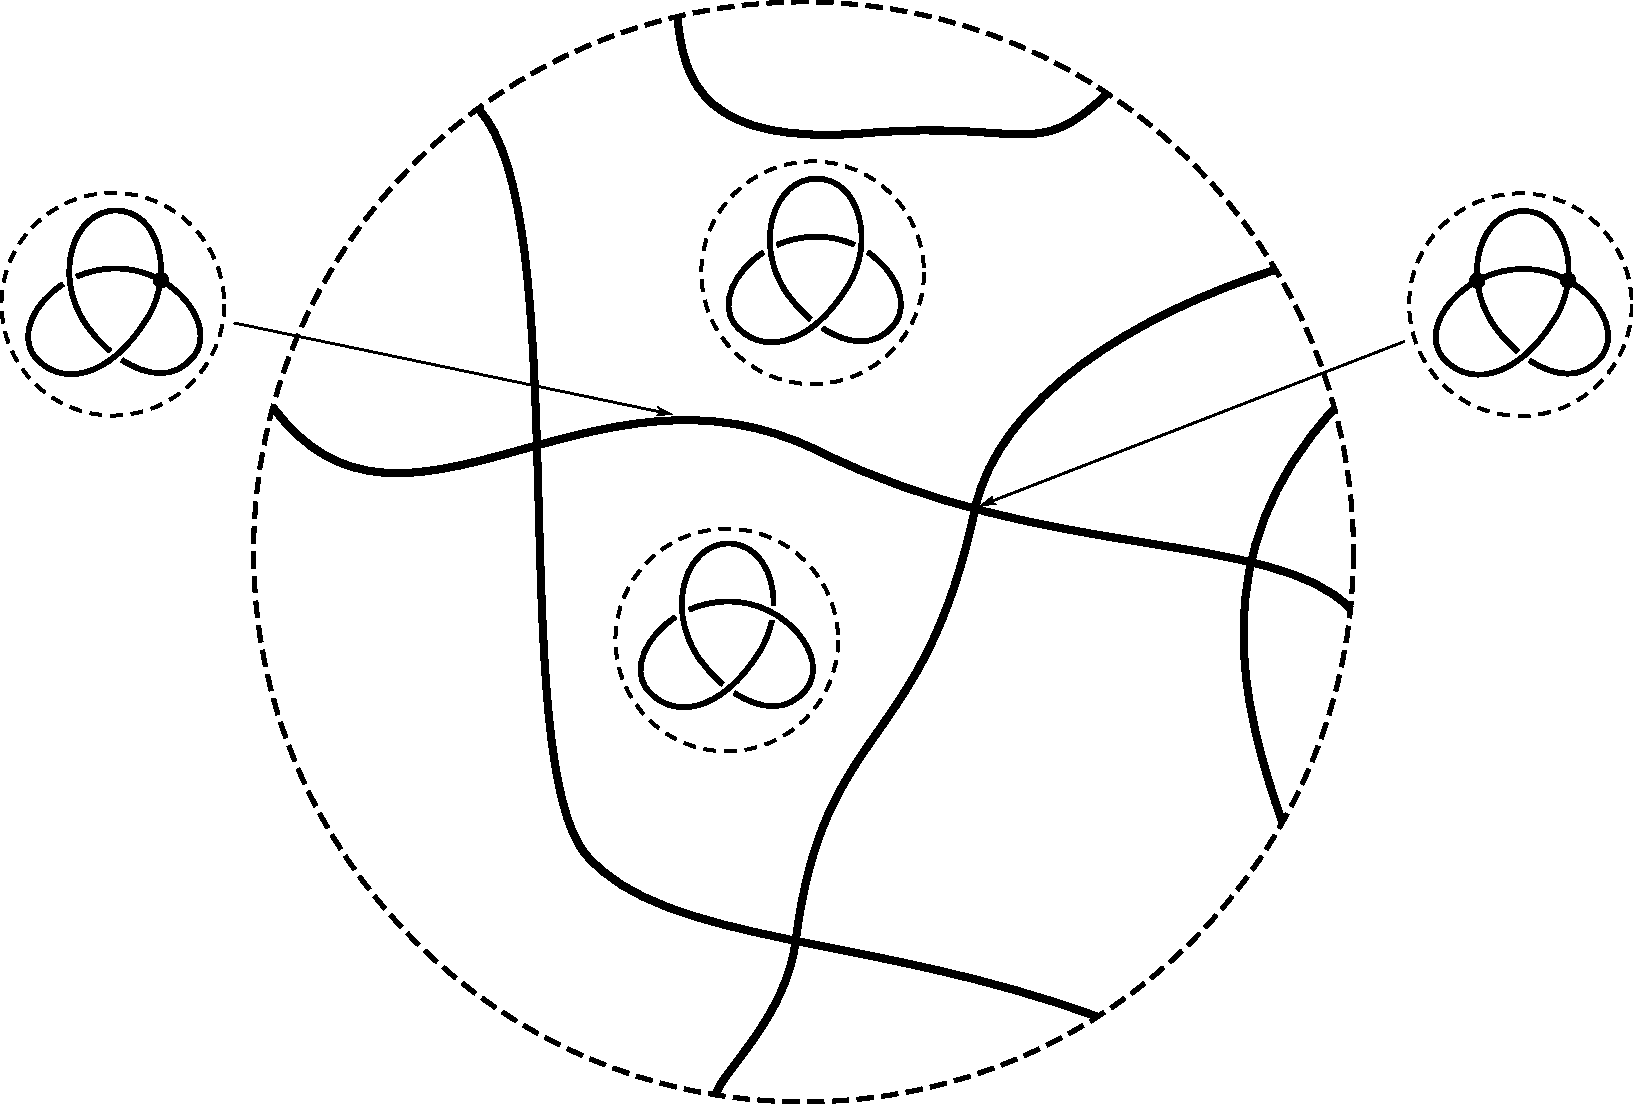
\includegraphics[width=0.55\linewidth]{stratification.pdf}
\end{center}

\begin{mdframed}
	In \cite{cohomology-of-knot-spaces}, Vassiliev makes a sequence of approximations of the cohomology ring of the space of knots, yielding a certain subring of the zeroth cohomology ring. Elements of the zeroth cohomology are locally constant functions on the space, so knot invariants. The invariants in this ``Vassiliev'' subring can be computed on any knot by some procedure involving the homology group of the strata at a finite number of increasing depths.

	Birman and Lin in \cite{knot-polynomials-and-vassilievs-invariants} give an axiomatic definition of the Vassiliev invariants as those that respect the Vassiliev skein relation. It follows, as we will see in Chapter \ref{ch:vassiliev-invariants-and-chord-diagrams} that Vassiliev invariants can be described completely combinatorially by functions on chord diagrams obeying certain combinatorial rules.

	By the work of Bar-Natan in \cite{on-the-vassiliev-knot-invariants} the algebra of chord diagrams turns out to be equivalent to a different diagrammatic algebra, that of Jacobi diagrams, again up to a different set of combinatorial rules. This will be discussed in Chapter \ref{ch:lie-theory-and-jacobi-diagrams}. This change of perspective introduces Lie theory in the following sense. A key relation in the algebra of Jacobi diagrams is a formal version of the relation in the universal enveloping algebra of a Lie algebra that the bracket is equal to the commutator. This is discussed in Chapter \ref{ch:jacobi-diagrams-as-a-universal-enveloping-algebra}. A rigorous version of this statement is the work of Hinnich and Vaintrob \cite{cyclic-operads-and-the-algebra-of-chord-diagrams} which constructs the algebra of Jacobi diagrams as the universal enveloping algebra object of some Lie algebra object in some tensor category.

	A paragraph introducing welded knots: If knots have to do with the configuration space of some number of points, then welded knots have to do with the configuration space of some number of `flying rings'. Arrowed Jacobi diagrams will need to be introduced. Kashiwara-Vergne may need to be mentioned.

	In Chapter \ref{ch:arrowed-jacobi-diagrams-as-a-universal-enveloping-algebra}, we generalise the result that Jacobi diagrams are a universal enveloping algebra to directed(/welded/arrowed) Jacobi diagrams.

	Some paragraphs talking about the rest of the Chapters.
\end{mdframed}


        \chapter{Vassiliev invariants and chord diagrams}
\label{ch:vassiliev-invariants-and-chord-diagrams}

\lettrine{\libertineInitialGlyph{V}}{assiliev} invariants are sophisticated to define in terms of the space of knots from the introduction, but the axiomatic definition of Birman-Lin \cite{knot-polynomials-and-vassilievs-invariants} is much simpler. The definition also illustrates an analogy first made by Bar-Natan \cite{on-the-vassiliev-knot-invariants} in which Vassiliev invariants are ``polynomial invariants''. This is not meant in the sense that Vassiliev invariants take values in a polynomial ring (like say, the Jones polynomial), but rather that Vassiliev invariants have special properties not shared by all invariants, just as polynomial functions have special properties not shared by all functions.

\section{Vassiliev Invariants}

\begin{definition}
	A \textbf{singular knot} is an immersion of \(S^{1}\) into \(\R^{3}\) which fails to be an embedding at finitely many singularities, and where the singularities are double-points and transverse. When a singular knot has \(m\) such singularities, we call it \textbf{\(m\)-singular}.
\end{definition}

\begin{remark}
	Knots with triple-points (and so on) are excluded from this definition, despite also being immersions with singularities.
\end{remark}

A singular knot with one double point is very close to two other knots, one where it's replaced by a positive crossing and one by a negative. If the conditions are right, we can extend a knot invariant to an invariant of singular knots by ``taking its derivative''.

\begin{definition}
	\label{def:derivative}
	The \textbf{derivative} \(\delta\) of a differentiable \(m\)-singular knot invariant \(f\) is
	\[\delta f \left( \double \right) = f \left( \poscross \right) - f\left( \negcross \right).\]
\end{definition}

What are the conditions? For this to be a well-defined operation, it mustn't matter which double point we choose.

\begin{definition}
	\label{def:differentiable-invariant}
	An invariant \(f\) of \(m\)-singular knots is \textbf{differentiable} if
	\begin{equation}
		f \left( \poscross \ \double \right) - f\left( \negcross \ \double \right) = f \left( \double \ \poscross \right) - f\left( \double \ \negcross \right).
	\end{equation}
\end{definition}

If an invariant of \(m\)-singular knots is differentiable, so is its derivative, so it can be extended to any number of double points.

Rather than thinking about functions on knots satisfying certain relations, the modern version of this subject takes the philosophy of imposing relations on the objects directly.

\begin{definition}
	\label{def:differentiability-relation}
	Define \(\mathcal{K}_{m} = \operatorname{span}(\{m\text{-singular knots}\})/\text{boundary relation}\),\\
	where the boundary relation is
	\[\poscross \ \double - \negcross \ \double = \double \ \poscross - \double \ \negcross.\]

	From now on, we will refer to elements \(\mathcal{K}_{m}\) as \(m\)\textbf{-singular knots}, and the DIFF relation will be implicit in everything.
\end{definition}

\begin{definition}
	\label{def:boundary}
	The \textbf{boundary} operation is the map \(\partial : \mathcal{K}_{m} \to \mathcal{K}_{m - 1}\) defined by
	\[ \double \longmapsto \poscross - \negcross .\]
\end{definition}

\begin{remark}
	The definitions \ref{def:derivative} and \ref{def:differentiable-invariant} are dual to \ref{def:differentiability-relation} and \ref{def:boundary}. For example, a differentiable invariant of knots is the same as a invariant of knots in \(\mathcal{K}_{m}\).
\end{remark}

Any knot invariant, \(f\) can be extended to an invariant \(f^{(m)}\) of \(m\)-singular knots by the Vassiliev skein relation
\[f^{(0)} = f\]
and
\[f^{(m + 1)}\left(\double\right) = f^{(m)}\left(\poscross\right) - f^{(m)}\left(\negcross\right).\]
Often, we omit the superscript and write
\[f\left(\double\right) = f\left(\poscross\right) - f\left(\negcross\right).\]

The Vassiliev skein relation extends a knot via its derivative, or chooses a value on \((m + 1)\)-singular knots to agree with the difference of values on its boundary.

% TODO: Could move later, even.
\begin{definitions}
	\begin{enumerate}[(a)]
		\item A knot invariant \(V\) is a \textbf{Vassiliev invariant} of order (or type) \(m\) if when extended to singular knots via the Vassiliev skein relation, there is an integer \(m\) such that
		\[V\biggl( \underbrace{\double \cdots \double}_{{\scriptscriptstyle m + 1}} \biggr) = 0.\]
	\item The \textbf{order} of a Vassiliev invariant \(V\) it the highest \(m\) such that \(V\) is a Vassiliev invariant of order \(m\). (That is, the order of a Vassiliev invariant is the highest number of double points a knot \(K\) can have without \(V(K)\) having to vanish).
	\end{enumerate}
\end{definitions}

\begin{remark}
	Vassiliev invariants of order \(m\) are those that vanish after \(m + 1\) derivatives, just like degree \(m\) polynomials.
\end{remark}

There are many other similar remarks to be made about the analogy between Vassiliev invariants and polynomials. To help see the bird's eye view, and following \cite{integration-of-singular-braid-invariants}, we phrase this in terms of an integration theory.

\begin{definition}
	An \textbf{integration theory} is a sequence
	% https://q.uiver.app/#q=WzAsNixbMSwwLCJcXG1hdGhjYWx7T31fe219Il0sWzAsMCwiXFxjZG90cyJdLFsyLDAsIlxcbWF0aGNhbHtPfV97bSAtIDF9Il0sWzMsMCwiXFxjZG90cyJdLFs0LDAsIlxcbWF0aGNhbHtPfV97MX0iXSxbNSwwLCJcXG1hdGhjYWx7T31fezB9Il0sWzEsMCwiXFxwYXJ0aWFsIl0sWzAsMiwiXFxwYXJ0aWFsIl0sWzIsMywiXFxwYXJ0aWFsIl0sWzMsNCwiXFxwYXJ0aWFsIl0sWzQsNSwiXFxwYXJ0aWFsIl1d
	\[\begin{tikzcd}
		\cdots & {\mathcal{O}_{m}} & {\mathcal{O}_{m - 1}} & \cdots & {\mathcal{O}_{1}} & {\mathcal{O}_{0}}
		\arrow["\partial", from=1-1, to=1-2]
		\arrow["\partial", from=1-2, to=1-3]
		\arrow["\partial", from=1-3, to=1-4]
		\arrow["\partial", from=1-4, to=1-5]
		\arrow["\partial", from=1-5, to=1-6]
	\end{tikzcd}\]
	of abelian groups. Note that we do not assume \(\partial^{2} = 0\).
\end{definition}

The group is \(\mathcal{O}_{0}\) is typically free abelian, and in our case is the primary object we want to study. The groups \(\mathcal{O}_{m}\) are also typically free abelian groups, and can often be thought of as \(m\)-singualr objects of some kind. The map \(\partial\) takes an \(m\)-singular object \(x\) to some combination of \((m - 1)\)-singular objects near \(x\).

By fixing an abelian group \(G\) and setting \(\mathcal{O}_{m}^{\ast} = \operatorname{Hom}(\mathcal{O}_{m}, G)\), we get the sequence
% https://q.uiver.app/#q=WzAsNixbMSwwLCJcXG1hdGhjYWx7T31fe219XntcXGFzdH0iXSxbMCwwLCJcXGNkb3RzIl0sWzIsMCwiXFxtYXRoY2Fse099X3ttIC0gMX1ee1xcYXN0fSJdLFszLDAsIlxcY2RvdHMiXSxbNCwwLCJcXG1hdGhjYWx7T31fezF9XntcXGFzdH0iXSxbNSwwLCJcXG1hdGhjYWx7T31fezB9XntcXGFzdH0iXSxbMCwxLCJcXGRlbHRhIiwyXSxbMiwwLCJcXGRlbHRhIiwyXSxbMywyLCJcXGRlbHRhIiwyXSxbNCwzLCJcXGRlbHRhIiwyXSxbNSw0LCJcXGRlbHRhIiwyXV0=
\[\begin{tikzcd}
	\cdots & {\mathcal{O}_{m}^{\ast}} & {\mathcal{O}_{m - 1}^{\ast}} & \cdots & {\mathcal{O}_{1}^{\ast}} & {\mathcal{O}_{0}^{\ast}}
	\arrow["\delta"', from=1-2, to=1-1]
	\arrow["\delta"', from=1-3, to=1-2]
	\arrow["\delta"', from=1-4, to=1-3]
	\arrow["\delta"', from=1-5, to=1-4]
	\arrow["\delta"', from=1-6, to=1-5]
\end{tikzcd}\]
where \(\delta\) is the transpose of \(\partial\).


% TODO: Integration constants (chord diagrams). We then ask if there are any relations. Explain this in terms of path "integrals". Say that if we find any relationship the functionals have to satisfy, we would should impose relations on objects rather than on functions.

\section{Second section}

\section{Third subsection}


        \chapter{Lie Theory and Jacobi Diagrams}
\label{ch:lie-theory-and-jacobi-diagrams}

% The following sections are simply a list of topics.

\section{(Rooted) Jacobi Diagrams}

\section{Floating Jacobi Diagrams}

\scaffold{In the next section we construct the suprising isomorphism between these two spaces.}

\section{PBW Theorem}

\scaffold{The Poincare-Birkhoff-Witt theorem for Lie algebras has many forms. One of these is that [...] . A corollary of this theorem \cite{enveloping-algebras} is that there is a `canonical' (though, not natural) isomorphism \(S(\mathfrak{g}) \to \mathcal{U}(\mathfrak{g})\) given by \[\omega(x_{1} \cdots x_{n}) = \frac{1}{n!} \sum_{\sigma \in S_{n}} x_{\sigma(1)} \cdots x_{\sigma(n)}.\] Which simply exhibits that fact that \(\operatorname{gr} A \cong A\) unnaturally.}

\scaffold{Futher, \cite{enveloping-algebras}, the two spaces (though not isomorphic as algebras) are isomorphic as \(\mathfrak{g}\)-modules: \(\mathcal{U}(\mathfrak{g})^{\mathfrak{g}} \cong S(\mathfrak{g})^{\mathfrak{g}}\).}

\scaffold{The following theorem is a diagrammatic version of the above.}

\section{Product, Coproduct and Hopf Algebra Structure}

\subsection{Primitive and Grouplike Elements}

\section{Vassiliev Invariants From Lie Algebras with a Metric}


        \chapter{Jacobi Diagrams as a Universal Enveloping Algebra}
\label{ch:jacobi-diagrams-as-a-universal-enveloping-algebra}

% Simply a list of topics to cover

\section{Operands and PROPs}

\section{What kinda monoidal category are we in?}

\section{Lie Algebra Objects}

\section{Metrics and Casimir Lie Algebras}

\section{Enveloping Algebras}

\section{External Enveloping Algebra, Internal Enveloping Algebra (?)}

% Testing italic text vs math

\(a b c d \text{   \textit{a b c d abcd}}\)



        \chapter{Welded Knots and Arrow Diagrams}
\label{ch:welded-knots-as-arrow-diagrams}

% Simply a list of topics

Question for myself: How does the integration theory change when welded crossings are involved?

\section{Welded knots and spinning}

\section{Arrow diagrams}


        \chapter{Arrowed Jacobi diagrams as a universal enveloping algebra}

\section{First subsection}

\section{Second section}

\section{Third subsection}


        \chapter{Expansions and associators}

\section{First subsection}

\section{Second section}

\section{Third subsection}


        \chapter{Emergent knotting}

\section{First subsection}

\section{Second section}

\section{Third subsection}


        \chapter{Emergent Welded Associators}
\label{ch:emergent-welded-associators}


        \appendix
        \titleformat{\chapter}[display]
        {\normalfont\bfseries\LARGE}
        {\chaptertitlename~\thechapter}
        {0pc}
        {{\color{black!30!white}\titlerule[0.7pt]}{\color{white}\titlerule[0.7pt]}{\color{black!30!white}\titlerule[0.7pt]}\vspace{0.8pc}\normalfont\Large}

        % \chapter{appendixname}
        % This is the first appendix.

        \emergencystretch=1em
        \newpage
        \printbibliography[title=References]


\end{document}
